\section{Experimental Evaluation}
\label{sec:results}

We have gathered preliminary performance results using a prototype
implementation of \pdht running on the Portals reference
implementation~\cite{portals-code}.  Results were gathered on the Comet
system at the San Diego Supercomputer Center with access provided
through the Extreme Science and Engineering Discovery Environment (XSEDE)
program.  Comet contains nodes with several configurations; for our
experiments, we used the Intel\regtm Xeon\regtm E5 nodes.  There are 1944 such
nodes, which are constructed from Dell\othertm PowerEdge\othertm C6320 servers
containing dual 12-core Intel\regtm Xeon\regtm E5-2680 processors and 128
gigabytes of memory.  Nodes are connected using a Mellanox\othertm FDR 56 Gb/s
InfiniBand\othertm fabric.

An initial study of the performance of \pdht can be seen in
Figure~\ref{fig:throughput}. This figure shows that \pdht scales
reasonably, with communication volume increasing as processor counts
grow. This experiment was run on one core per node, with the hash
function configured to ensure all reads occur remotely, over the
Infiniband\othertm interface.

Additionally, we measure the performance of retrieving elements
from the \pdht in different scenarios.  These results are shown in
Figure~\ref{fig:mlen} and provide an initial characterization of the lookup
cost associated with our \pdht implementation.  In contrast with traditional
PGAS approaches, building a remotely accessible key/value store on top of a
mechanism intended to support MPI message matching can add new overheads.  In
particular, the Portals message processing engine must traverse the active
match list until an ME that matches the given query is located.  In cases where
the element does not exist, the Portals layer must reach the end of the list to
make this conclusion.  Thus, there is a list traversal overhead that is
proportional to the number of elements visited before finding a match.

\begin{figure}
    \centering
    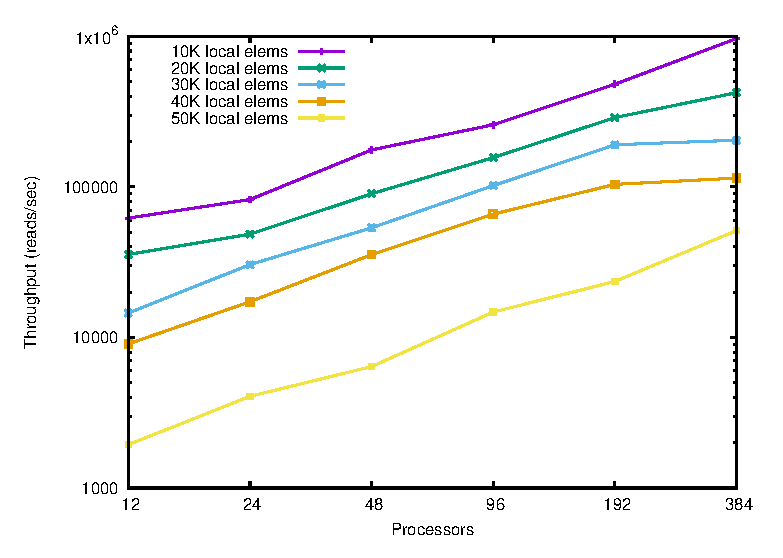
\includegraphics[width=\linewidth]{plots/throughput}
    \caption{System throughput for a range of local volume (entries per node).}
    \label{fig:throughput}
\end{figure}

\begin{figure}
    \centering
    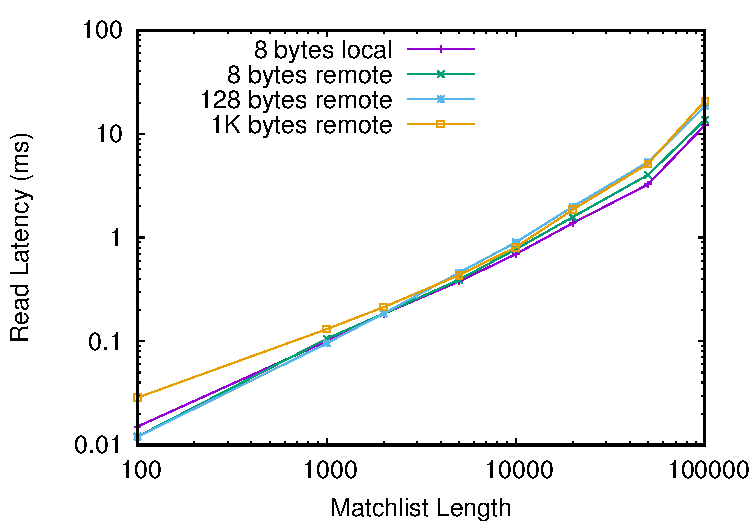
\includegraphics[width=\linewidth]{plots/mlen}
    \caption{Read operation latency versus list depth for various size entries.}
    \label{fig:mlen}
\end{figure}

The Portals layer must maintain each matching list as an ordered list in order
to preserve MPI message ordering semantics.  However, we observe that this
ordering is not required by \pdht.  Also, in contrast to MPI applications,
where typical communication patterns result in short matching lists or in
matching occurring near the head of the list, \pdht necessarily generates long
matching lists with an expected matching depth of the midpoint in the list.
Thus, we identify this overhead as a key challenge to supporting such models
and plan to investigate solutions in our future work.

%%% Local Variables:
%%% mode: latex
%%% TeX-master: "paper"
%%% End:
